\chapter{Applied Machine Learning for classification problems in Chemistry}
\section{Introduction}
Like in magnetic resonance, majority of early developed models such as first description of perceptron or simple neuron were done by McCulloh and Pitts in 1943\cite{McCulloch1943} but were not used due to the lack of computational power. With rise of distributed computing specifically in this decade field of Artificial Intelligence gain a significan boost with Graphical Processing Unit (GPU) computations decreasing in some cases training of extensive machine learning models from monthes to simply hours with minimum cost involved. This simply greatly impacted variety of applications of ML to solve actual real world problems such as fracture detection from X-ray images\cite{Tian2003} or cancer prediction using gene expression profiling\cite{khan:2001}. Machine Learning models are divided in two groups: Supervised and Unsupervised. Supervised models are such models that require labled data from which they "learn" data in order to be able predict label for the newly introduced data. Typicaly this are Arificial Neural Networks, Support Vector Machines and etc. Unsupervised models are trying to gather insight from the data and group it accordingly to self-defined class or labels, intuitively this are clustering models such as hierrarhical or k-means algorithms. Widely for some problems unsupervised models are used fo prprocessing to perform demensionality reduction in order to fight curse of dimensionality, when extra-features can reduce greatly the predictive power. In this work we will specifically work with supervised models and some unsupervised algortihms were used for geature selection. In this chpater we will discuss how one can use Support Vector Machines, Arificial Neural Networks, Genetic Algorithms and their limitations. We will also discussed bottlenecks that we have faced during this work such as overfitting after preprocessing and etc. 
\subsection{Support vector Machines}
Support Vector Machines(SVMs) is a really well known and used supervised machine learning technique for data classification. It was first developed by Vladimir Vapnik an soviet expatriate to United States who worked at that time for AT\& T Bell Labs. In a simply few words idea of SVMs is to linearly separate the data which might be non-linearly separable. I will touch main aspects of theoretical derivation to understand the idea behind SVM and will not dive into mathematical madness.
Lets assume that $X$ is a feature space or space of an objects, and $Y$ is a set of solutions. It is obvious that an algorithm that will find approximate dependencies between the feature $X$-space and the solution $Y$-space have to be found in form $F:X\rightarrow Y$.  At the moment lets only deal with binary classification    namely $Y=(-1,+1)$ and feature space is described by $n$-dimensional real vectors $X=\mathbf{R}^n$. 
The classifier will have the form: 
\begin{equation}\label{eq:svm}
F(x)=sign(\sum_{j=1}^{n} \omega_j x_j-\omega_0)=sign(x^{T}\omega-w_0)
\end{equation}
Where $x=(x_1,....,x_n)$- evidential description of an object $X$ whose transpose should be taken; vector $\omega=(\omega_1,....,\omega_n)$ and value of $\omega_0$ are some parameters of the algorithm. And sign of the sum will define to which class corresponds the given feature. If sign is negative solution is $Y=-1$ and if it returns positive $Y=1$. Taking away $sign$ Eq.\ref{eq:svm} defines a hyperplane which has 2 dimensions in a 3-D space and 1-D in a 2-D space. The idea is to generate family of hyperplanes until one that creates biggest margin between training points is found. That means appropriate $\omega$ and $\omega_0$ have to be determined for the specific data set. An example of is give on Fig.\ref{figure:svm1}    
\begin{figure}[h!]
\centering
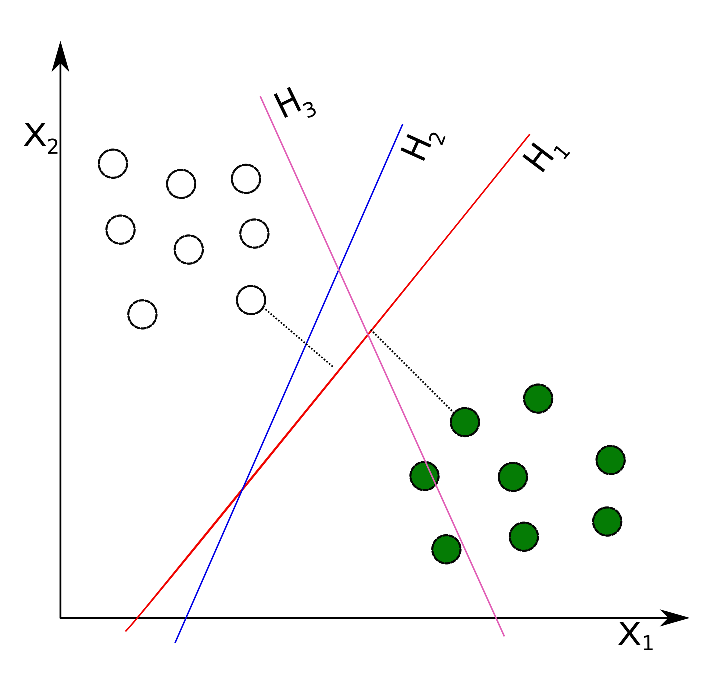
\includegraphics[width=1\textwidth]{figures/chap3/svm1.eps}
\caption{}
\label{figure:svm1}
\end{figure}
If we assume that data set is linearly separable one can define an error function of training as: 
\begin{equation}
Q(\omega,\omega_0)=\sum_{i=1}^l[y_i(\langle \omega,x_i\rangle-\omega_0)<0]
\end{equation}
Conditions on the border: 
\begin{equation}\label{eq:svmb1}
\omega,x_i\rangle-\omega_0=y_i
\end{equation} 
and 
\begin{equation}\label{eq:svmb2}
\langle \omega,x_i\rangle-\omega_0 = \begin{cases} \leq-1, & \mbox{if } y_i=-1 \\ \geq1 , & \mbox{if } y_i=1 \end{cases}
\end{equation}
From Eq.\ref{eq:svmb1} and Eq.\ref{eq:svmb2} it is obvious that hyperplane should be tied by the condition: 
\begin{equation}\label{eq:svmb3}
-1<\langle \omega,x\rangle-\omega_0<1
\end{equation}
It is pretty obvious that separation width between to classes can be defined as $\frac{2}{||\omega||}$ and it is more clear on Fig.\ref{figure:svm2}.  
\begin{figure}[h!]
\centering
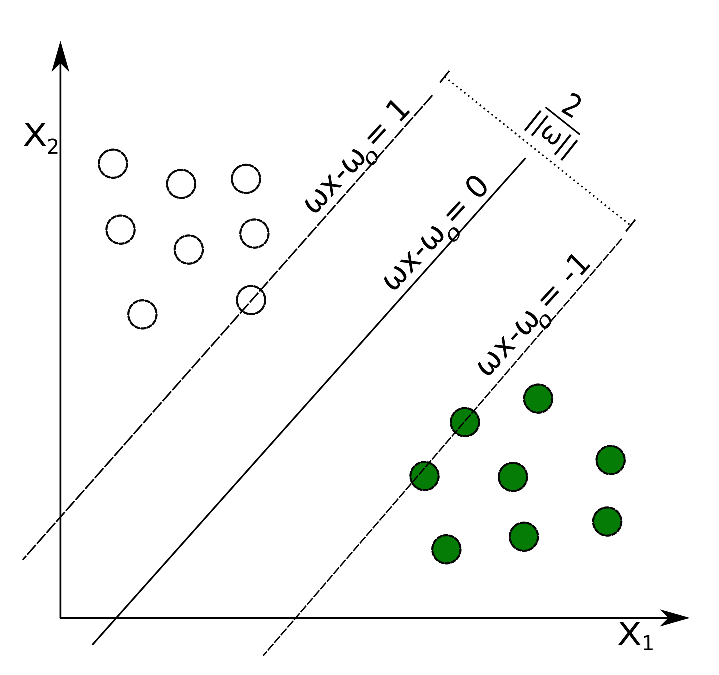
\includegraphics[width=1\textwidth]{figures/chap3/svm2.eps}
\caption{}
\label{figure:svm2}
\end{figure}
If data is perfectly linearly separable then $||\omega||^2$ can be minimized by two constraints: 
\begin{equation}
\begin{cases} \langle \omega,\omega\rangle \rightarrow min;\\ y_i(\langle \omega,x_i\rangle-\omega_0)\geq1 , &  y=1,...,l  \end{cases}
\end{equation}
In more compact form:
\begin{equation}\label{eq:svmconst}
y_i(\omega\cdot x_i+\omega_0)\geq 1
\end{equation}
If features of two classes are allowed to overlap and no longer linear separability is presented it is possible to allow some points to appear on the other or wrong side of margin and to add slack variables such as $\xi=(\xi_1,\xi_2,...,\xi_N)$ or thus constraint from Eq.\ref{eq:svmconst} can be written as: 
\begin{equation}\label{eq:svmconst}
y_i(\omega\cdot x_i+\omega_0)\geq 1-\xi_i, \xi_i\geq 0
\end{equation}
And thus minimization problem is given as $||\omega||^+C\sum_{i=1}^m\xi_i$ where $C$ is an adjustable parameter known as "cost". \\* 
Computationally and algorithmically problem converges to the convex optimization search of quadratic  terms with the linear constraints and methods can be find elsewhere in the literature \cite{book}. Using Kuhn-Tucker conditions the solution of the problem above diverge to the problem of Lagrange function saddle point and classification algorithm can be rewritten as:
\begin{equation}\label{eq:svmg}
F(x)=sign(\sum_{i=1}^{N} \lambda_iy_i\langle x_i,x\rangle-\omega_0)
\end{equation}
Solution for $\omega$ now is given as: 
\begin{equation}
\omega=sign(\sum_{i=1}^{N} \lambda_iy_ix_i
\end{equation}
If $\lambda_i$ are nonzero coefficients for the $i$-th observation and it will compromise the constraint thus this observation is called a support vector. \\*
\begin{figure}[h!]
\centering
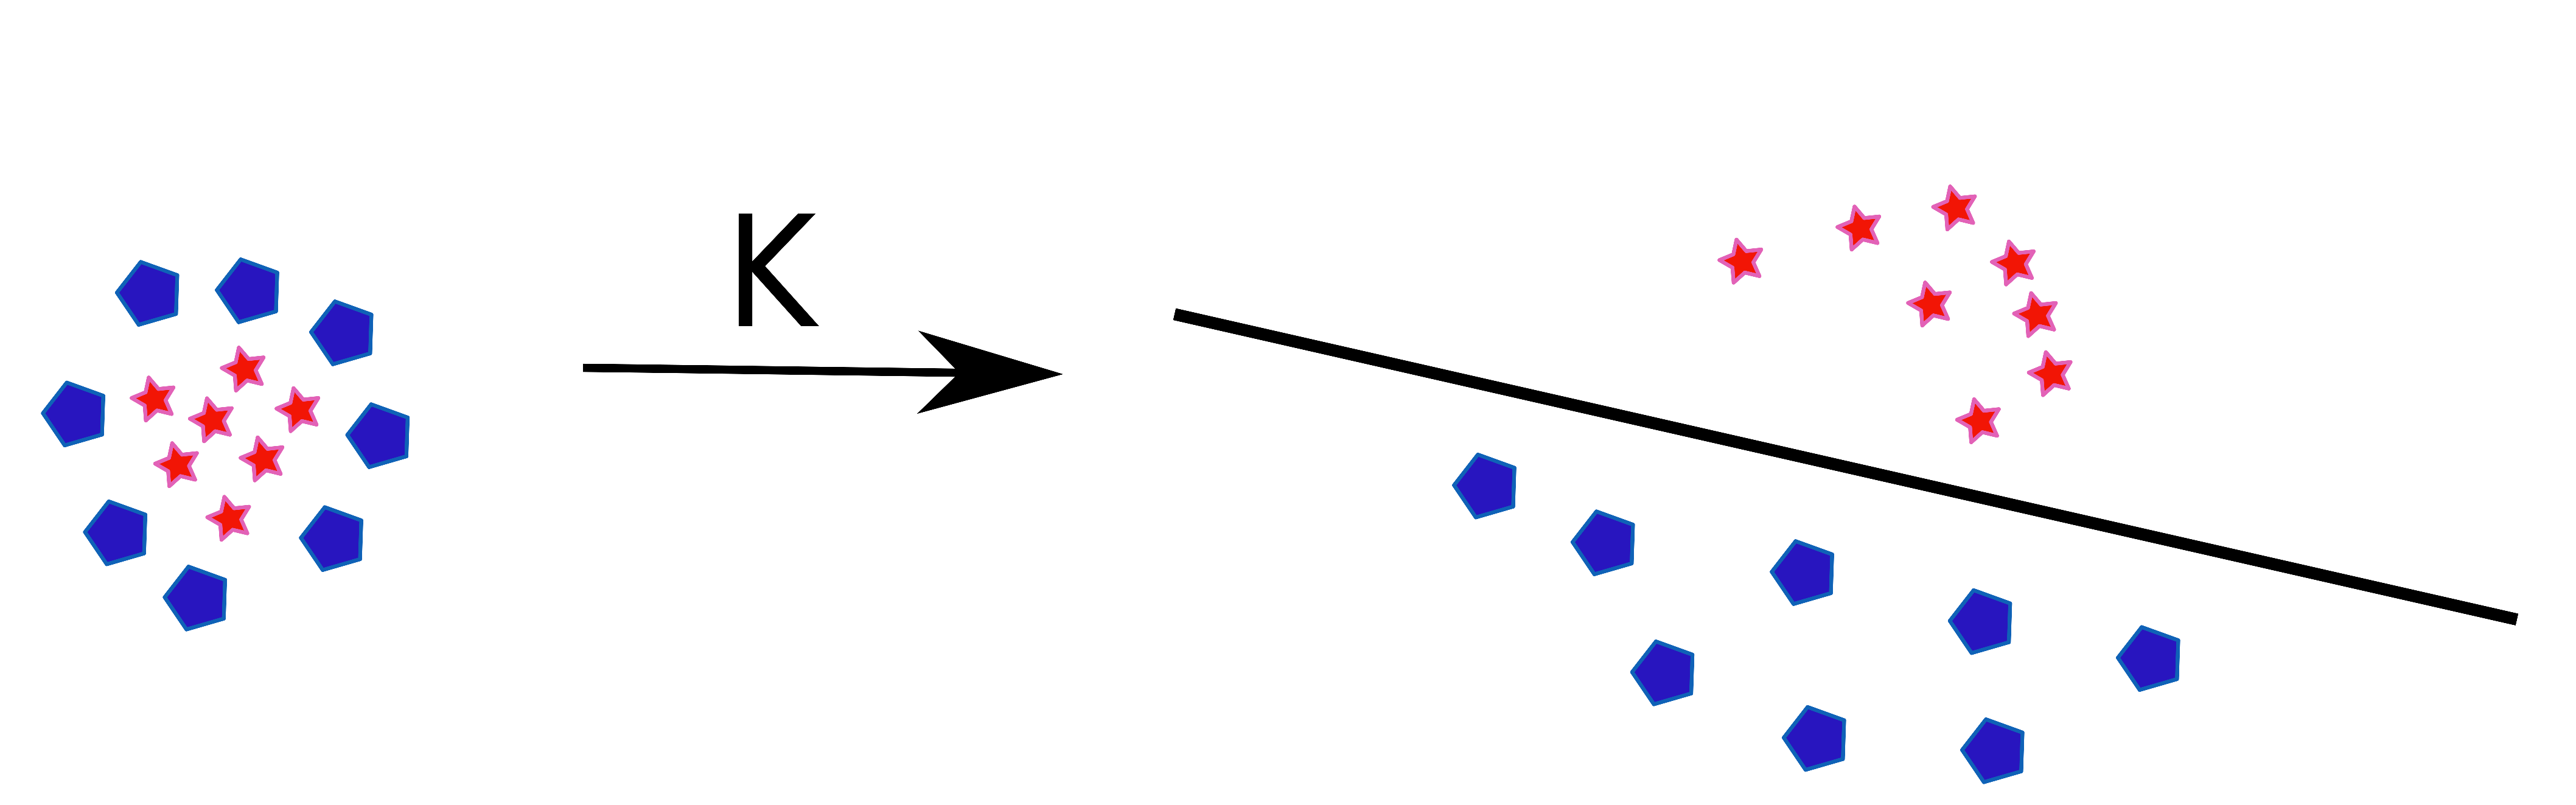
\includegraphics[width=1\textwidth]{figures/chap3/bound.eps}
\caption{}
\label{figure:svm2}
\end{figure}
If the boundaries are no longer linear as an example on Fig.\ref{figure:bound} then a new feature space should be introduced. That transformation is the cause of such popularity of SVMs among data analyst community. It can be done using kernel functions that map original data into the new feature space that is now is capable of hyperplane separation of the classified data. Eq.\ref{eq:svmg} can be modified a bit: 
\begin{equation}\label{eq:svmg}
F(x)=sign(\sum_{i=1}^{N} \lambda_iy_iK(x_i,x)-\omega_0)
\end{equation} 
Where $K(x_i,x)$ is the kernel and it should be chosen as symmetric and positive definite or semi-definite function or simply satisfy Mercer condition~\cite{mercer}. There are two most popular choices of the $K$ function: 
\begin{description} \item[Polynomial] $K(x,x')=(1+\langle x,x'\rangle)^d$ \item[Radial basis]$K(x,x')=exp(-\gamma||x-x'||^2)$  \end{description}
The first choice is more computationally cost efficient and numerically unstable when $d$ is increasing. For $d=1$ polynomial kernel reduces to original linear and most common is the quadratic when $d=2$. Radial kernel is an example of transformation of data to infinite dimensional Hilbert space(commonly hypersphere). $\gamma$ in exponent is known as kernel bandwidth and it is one of the tunable and boosting parameters for training the classifier. It is much more widely common to use in the data scientists community. SVM used as binary classifier and multi-class problems usually performed using either each against all method and taking the best score($n$ binary classification problems) or all against each other($n(n-1)/2$ binary classification problems). Most out of box methods do support multi-class classification in R, Python but not in Matlab which can be done easily.  In our work results for both type of kernels will be presented and compared.           
\clearpage
\subsection{Artificial Neural Networks}

